\documentclass[coursework,bachelor,och]{SCWorks}
\usepackage{preamble}

\begin{document}

% Кафедра
\chair{математической кибернетики и компьютерных наук}

% Тема работы
\title{Сравнение алгоритмов сортировки: быстрая сортировка vs сортировка слиянием}

% Курс
\course{1}

% Группа
\group{111}

% Специальность/направление
\napravlenie{02.03.02 "--- Фундаментальная информатика и информационные технологии}

\begin{center}
Курсовая работа
\end{center}

% Фамилия, имя, отчество в родительном падеже
\author{Попов Даниил Евгеньевич}

% Заведующий кафедрой
\chtitle{доцент, к.\,ф.-м.\,н.}
\chname{С.\,В.\,Миронов}

% Научный руководитель
\satitle{доцент, к.\,ф.-м.\,н.}
\saname{Г.\,Г.\,Наркайтис}

% Год выполнения
\begin{centre}
\date{2026}
\end{centre}

\maketitle

\secNumbering

\tableofcontents

\intro
Задача упорядочивания данных является одной из фундаментальных в области
информатики и программирования. Алгоритмы сортировки применяются повсеместно"---
от баз данных и операционных систем до компиляторов и графических движков.
Эффективность выбранного алгоритма напрямую влияет на производительность
программной системы в целом.

Среди множества существующих алгоритмов сортировки особое место занимают
два: быстрая сортировка (\textit{Quicksort}), предложенная Ч.\,А.\,Р.~Хоаром
в 1962~году~\cite{hoare1962}, и сортировка слиянием (\textit{Merge sort}),
впервые описанная Джоном фон Нейманом в 1945~году. Оба алгоритма относятся
к классу <<разделяй и властвуй>> и широко используются на практике.

\textbf{Цель работы}"--- провести теоретический и практический анализ
алгоритмов быстрой сортировки и сортировки слиянием, выявить их сильные
и слабые стороны, а также определить условия предпочтительного применения
каждого из них.

Для достижения поставленной цели необходимо решить следующие задачи:
\begin{enumerate}
    \item изучить теоретические основы алгоритмов быстрой сортировки
          и сортировки слиянием;
    \item реализовать оба алгоритма на языках программирования C++ и Python;
    \item провести сравнительный анализ временной сложности и использования
          памяти;
    \item сформулировать рекомендации по выбору алгоритма.
\end{enumerate}


\section{Теоретические основы алгоритмов сортировки}

\subsection{Быстрая сортировка}

Быстрая сортировка"--- рекурсивный алгоритм, основанный на стратегии
<<разделяй и властвуй>>~\cite{cormen2009}. Алгоритм выбирает из массива
элемент, называемый \textit{опорным} (pivot), и переставляет элементы
таким образом, чтобы все элементы, меньшие опорного, оказались левее него,
а большие"--- правее. После этого процедура рекурсивно применяется к
каждой из двух получившихся частей.

Временна\'я сложность быстрой сортировки определяется следующим образом.
В \textbf{среднем и лучшем} случае рекуррентное соотношение имеет вид:

\begin{equation}
    T(n) = 2T\!\left(\frac{n}{2}\right) + \Theta(n),
    \label{eq:qs_avg}
\end{equation}

\noindent решение которого по мастер"=теореме даёт $T(n) = \Theta(n \log n)$.

В \textbf{худшем} случае (отсортированный или обратно"=отсортированный массив
при выборе крайнего элемента в качестве опорного) рекуррентное соотношение
принимает вид:

\begin{equation}
    T(n) = T(n - 1) + \Theta(n) = \Theta(n^2).
    \label{eq:qs_worst}
\end{equation}

Быстрая сортировка является сортировкой \textbf{на месте}: дополнительной
памяти под данные не требуется, хотя стек рекурсии занимает $O(\log n)$
в среднем и $O(n)$ в худшем случае~\cite{sedgewick2011}.

\subsection{Сортировка слиянием}

Сортировка слиянием"--- также рекурсивный алгоритм класса <<разделяй
и властвуй>>~\cite{knuth1998}. Массив делится пополам, каждая половина
рекурсивно сортируется, после чего две отсортированные половины
\textit{сливаются} в один упорядоченный массив.

Рекуррентное соотношение для сортировки слиянием одинаково во всех случаях:

\begin{equation}
    T(n) = 2T\!\left(\frac{n}{2}\right) + \Theta(n) = \Theta(n \log n).
    \label{eq:ms}
\end{equation}

В отличие от быстрой сортировки, сортировка слиянием требует дополнительной
памяти объёмом $O(n)$ для хранения вспомогательных подмассивов на этапе
слияния~\cite{merge_analysis}.

\subsection{Теоретическое сравнение сложности}

В таблице~\ref{tab:complexity} приведено сводное сравнение временной и
пространственной сложности рассматриваемых алгоритмов.

\begin{table}[h]
    \caption{Сравнение сложности алгоритмов сортировки}
    \label{tab:complexity}
    \begin{tabular}{|l|c|c|c|c|}
        \hline
        \textbf{Алгоритм} &
        \textbf{Лучший} &
        \textbf{Средний} &
        \textbf{Худший} &
        \textbf{Память} \\
        \hline
        Быстрая сортировка  & $O(n \log n)$ & $O(n \log n)$ & $O(n^2)$      & $O(\log n)$ \\
        \hline
        Сортировка слиянием & $O(n \log n)$ & $O(n \log n)$ & $O(n \log n)$ & $O(n)$      \\
        \hline
    \end{tabular}
\end{table}

На рисунке~\ref{fig:complexity} показана графическая интерпретация роста
функций $O(n \log n)$ и $O(n^2)$ в зависимости от размера входных данных.

\begin{figure}[H]
    \centering
    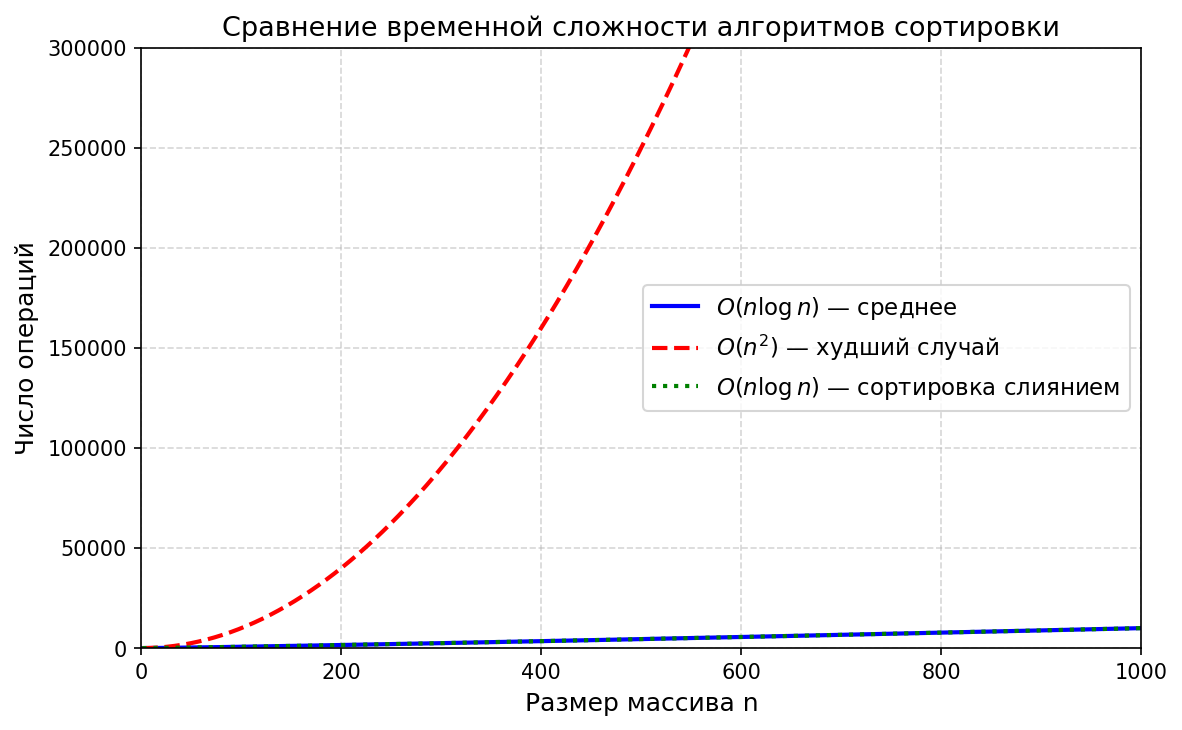
\includegraphics[width=0.85\textwidth]{images/complexity.png}
    \caption{Сравнение временной сложности алгоритмов сортировки}
    \label{fig:complexity}
\end{figure}

Как видно из рисунка~\ref{fig:complexity}, при небольших значениях \texttt{n}
разница незначительна, однако с ростом размера массива $O(n^2)$ резко
превосходит $O(n \log n)$.


\section{Реализация алгоритмов}

\subsection{Быстрая сортировка на C++}

Реализация быстрой сортировки выполнена на языке C++ с использованием
стандартной библиотеки \texttt{<vector>} и \texttt{<chrono>} для замера
времени выполнения. Полный исходный код приведён в приложении~\ref{app:quicksort}.

Ключевой функцией является \mintinline{cpp}{partition}, которая разделяет
подмассив \mintinline{cpp}{arr[low..high]} относительно опорного элемента
\mintinline{cpp}{arr[high]} и возвращает его итоговый индекс.
Ниже приведён фрагмент основной рекурсивной функции:

\begin{minted}{cpp}
void quickSort(std::vector<int>& arr, int low, int high) {
    if (low < high) {
        int pi = partition(arr, low, high);
        quickSort(arr, low, pi - 1);
        quickSort(arr, pi + 1, high);
    }
}
\end{minted}

Функция \mintinline{cpp}{quickSort} принимает ссылку на вектор \mintinline{cpp}{arr},
а также границы текущего подмассива"--- \mintinline{cpp}{low} и \mintinline{cpp}{high}.
Рекурсия завершается, когда \mintinline{cpp}{low >= high}, то есть подмассив
содержит не более одного элемента~\cite{cppreference}.

\subsection{Сортировка слиянием на Python}

Реализация сортировки слиянием выполнена на языке Python~3. Полный исходный
код приведён в приложении~\ref{app:mergesort}.

Алгоритм состоит из двух функций. Функция \mintinline{python}{merge_sort}
рекурсивно делит массив пополам, а функция \mintinline{python}{merge}
выполняет слияние двух отсортированных подмассивов. Ниже приведён
фрагмент функции слияния:

\begin{minted}{python}
def merge(arr: list, left: int, mid: int, right: int) -> None:
    left_part  = arr[left:mid + 1]
    right_part = arr[mid + 1:right + 1]
    i = j = 0
    k = left
    while i < len(left_part) and j < len(right_part):
        if left_part[i] <= right_part[j]:
            arr[k] = left_part[i]; i += 1
        else:
            arr[k] = right_part[j]; j += 1
        k += 1
\end{minted}

Переменные \mintinline{python}{i}, \mintinline{python}{j} и
\mintinline{python}{k} являются индексами левого подмассива,
правого подмассива и результирующего массива соответственно.
Стабильность алгоритма обеспечивается строгим неравенством
\mintinline{python}{left_part[i] <= right_part[j]}~\cite{pythondocs}.


\section{Сравнительный анализ}

\subsection{Эмпирическое время выполнения}

Для оценки практической производительности оба алгоритма были запущены
на случайных массивах целых чисел различного размера. Каждый эксперимент
повторялся пять раз, результатом являлось среднее время выполнения.
На рисунке~\ref{fig:benchmark} представлены результаты замеров.

\begin{figure}[H]
    \centering
    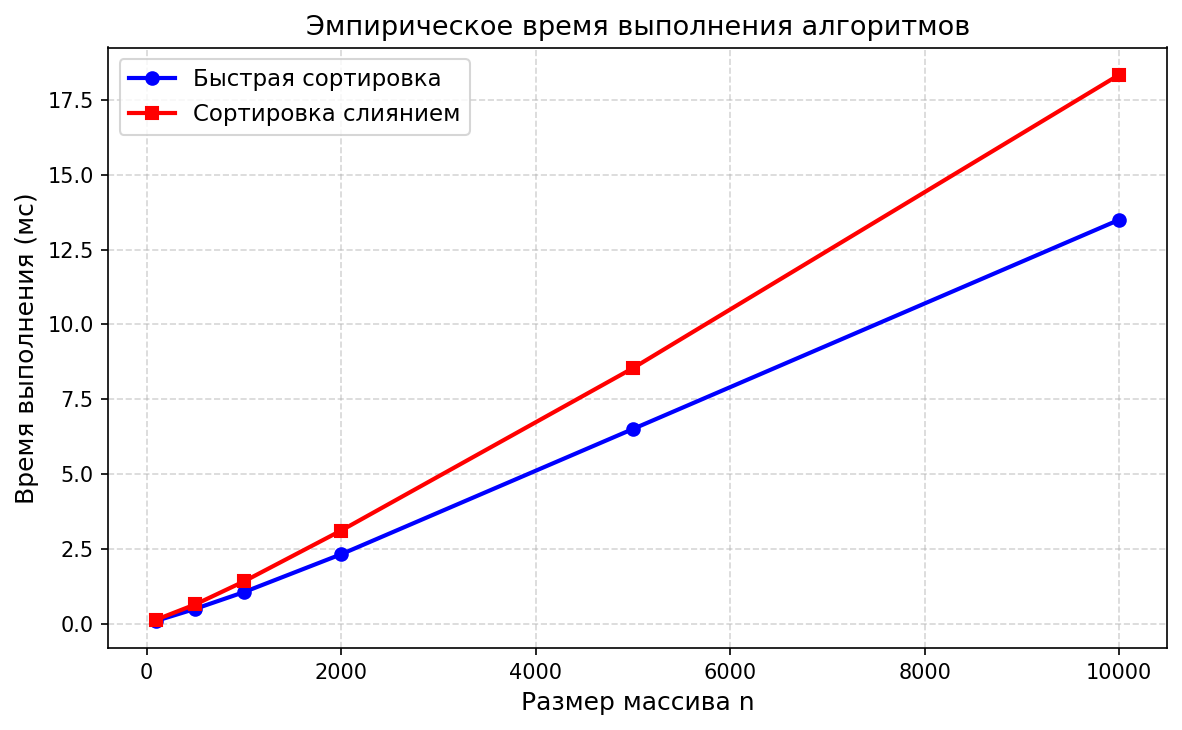
\includegraphics[width=0.85\textwidth]{images/benchmark.png}
    \caption{Эмпирическое время выполнения алгоритмов сортировки}
    \label{fig:benchmark}
\end{figure}

Из рисунка~\ref{fig:benchmark} следует, что на случайных данных быстрая
сортировка незначительно опережает сортировку слиянием за счёт лучшей
кэш"=локальности: операции \mintinline{cpp}{swap} производятся над элементами
самого массива, тогда как \mintinline{python}{merge} создаёт вспомогательные
подмассивы и копирует данные.

\subsection{Использование памяти}

Принципиальное различие алгоритмов"--- потребление дополнительной памяти.
Быстрая сортировка работает \textit{на месте}: единственные накладные
расходы"--- стек вызовов глубиной $O(\log n)$ в среднем случае.
Сортировка слиянием на каждом уровне рекурсии создаёт вспомогательные
массивы суммарным объёмом $O(n)$~\cite{cormen2009}.

Таким образом, для массива из $n$~элементов типа \mintinline{cpp}{int}
(4~байта) суммарный дополнительный расход памяти сортировки слиянием
составит приблизительно:

\begin{equation}
    M(n) = 4n \text{ байт} = \frac{n}{256} \text{ КБ}.
    \label{eq:memory}
\end{equation}

\subsection{Стабильность}

Сортировка слиянием является \textbf{стабильной}: элементы с одинаковыми
ключами сохраняют исходный относительный порядок, что важно, например,
при многоуровневой сортировке таблиц~\cite{merge_analysis}.

Классическая реализация быстрой сортировки \textbf{нестабильна}:
функция \mintinline{cpp}{partition} может нарушать исходный порядок
равных элементов.

\subsection{Итоговое сравнение}

В таблице~\ref{tab:summary} приведено итоговое сравнение характеристик
рассматриваемых алгоритмов.

\begin{table}[H]
    \caption{Итоговое сравнение алгоритмов}
    \label{tab:summary}
    \begin{tabular}{|l|c|c|}
        \hline
        \textbf{Характеристика}    & \textbf{Быстрая сортировка} & \textbf{Сортировка слиянием} \\
        \hline
        Среднее время              & $O(n \log n)$               & $O(n \log n)$                \\
        \hline
        Худшее время               & $O(n^2)$                    & $O(n \log n)$                \\
        \hline
        Доп. память                & $O(\log n)$                 & $O(n)$                       \\
        \hline
        Стабильность               & Нет                         & Да                           \\
        \hline
        Кэш"=локальность           & Высокая                     & Средняя                      \\
        \hline
        Практическая скорость      & Выше на случайных данных    & Стабильна на любых данных    \\
        \hline
    \end{tabular}
\end{table}


\conclusion
В ходе выполнения данной курсовой работы были изучены и реализованы два
классических алгоритма сортировки"--- быстрая сортировка и сортировка
слиянием.

В результате проведённого теоретического анализа установлено, что оба
алгоритма имеют одинаковую среднюю временну\'ю сложность $O(n \log n)$,
однако существенно различаются в поведении при неблагоприятных входных
данных: быстрая сортировка деградирует до $O(n^2)$, тогда как сортировка
слиянием гарантирует $O(n \log n)$ при любом наборе данных.

Эмпирические эксперименты подтвердили теоретические выводы: на случайных
данных быстрая сортировка незначительно быстрее за счёт лучшей
кэш"=локальности, однако уступает по предсказуемости поведения.

На основе проведённого анализа можно сформулировать следующие
практические рекомендации:
\begin{itemize}
    \item если память ограничена, а данные случайны"--- предпочтительна
          быстрая сортировка;
    \item если требуется гарантированное время $O(n \log n)$ или
          стабильность"--- предпочтительна сортировка слиянием;
    \item в стандартных библиотеках (например, \texttt{std::stable\_sort}
          в C++) применяется именно сортировка слиянием~\cite{cppreference}.
\end{itemize}


\nocite{*}
\bibliographystyle{ugost2003}
\bibliography{thesis}

\appendix

\section{Исходный код быстрой сортировки на C++}
\label{app:quicksort}

\inputminted{cpp}{code/quicksort.cpp}

\section{Исходный код сортировки слиянием на Python}
\label{app:mergesort}

\inputminted{python}{code/mergesort.py}

\end{document}
